\documentclass[12pt]{article}

% Font setup
\usepackage[T1]{fontenc}
\usepackage{mathpazo}  % Palatino-like font (similar to Garamond)
\usepackage{eulervm}   % Better matching math font

% Math packages (consolidated)
\usepackage{amsmath}
\usepackage{amssymb}
\usepackage{amsthm}
\usepackage{amsfonts}
\usepackage{amscd}
\usepackage{mathrsfs}
\usepackage{bm}
\usepackage[mathscr]{eucal}
\allowdisplaybreaks[4]

% Graphics and colors
\usepackage{graphicx}
\usepackage{color}
\usepackage{float}
\usepackage{epstopdf}

% Tables
\usepackage{dcolumn}
\usepackage{nicematrix}

% TikZ
\usepackage{tikz}
\usetikzlibrary{decorations.pathreplacing, matrix}

% Diagrams
\usepackage[all]{xy}  % Only included once now

% Special symbols
\usepackage{eurosym}
\usepackage{verbatim}

% Young tableaux
\usepackage{youngtab}
\usepackage{ytableau}
\ytableausetup{mathmode, boxsize=0.9em}

% Citation
\usepackage{cite}

% Hyperref (always load last)
\usepackage{hyperref}
\hypersetup{
    colorlinks=true,
    linkcolor=blue,
    citecolor=red,
    backref=page
}


\setlength{\evensidemargin}{0.3cm}
\setlength{\oddsidemargin}{1.5cm}
\parskip=6pt
\frenchspacing
\textwidth=15cm
\textheight=23cm
\parindent=16pt
\oddsidemargin=0.5cm
\evensidemargin=0.5cm
\topmargin=-1.2cm

% Theorem styles
\theoremstyle{definition}  % Set style to definition for all
\newtheorem{thm}{Theorem}[subsection]
\newtheorem{defi}[thm]{Definition}
\newtheorem{lemma}[thm]{Lemma}
\newtheorem{prop}[thm]{Proposition}
\newtheorem{coro}[thm]{Corollary}
\newtheorem{conj}[thm]{Conjecture}
\newtheorem*{pf}{Proof}  % Unnumbered Proof


% \theoremstyle{remark}
\newtheorem{ex}[thm]{Example}
\newtheorem{remark}[thm]{Remark}

% Problem environment (uses separate counter)
\newtheorem{prob}{Problem}[subsection]

% Equation numbering
\numberwithin{equation}{subsection}

\newcommand{\multichoose}[2]{\left(\!\middle(\vphantom{n}\genfrac{}{}{0pt}{}{#1}{#2}\middle)\!\right)}%multichoose symbol


\def\theequation{\thesection.\arabic{equation}}
\makeatletter \@addtoreset{equation}{section} \makeatother
\makeindex \setcounter{tocdepth}{2}
\def\qed{\hfill \rule{4pt}{7pt}}
\def\pf{\vskip 0.2cm {\noindent \bf Proof.}\quad}
\def\rank{\mbox{\rm rank}}
\def\corank{\mbox{\rm corank}}
\def\Im{\mbox{\rm Im}}
\def\id{\mbox{\rm id}}
\def\Poin{\mbox{\rm Poin}}
\def\Int{\mbox{\rm Int}}
\def\Nul{\mbox{\rm Nul}}
\def\nul{\text{Nul}}
\def\gcd{\mbox{\rm gcd}}
\def\lcm{\mbox{\rm lcm}}
\def\rk{\operatorname{rk}}
\def\res{\mbox{\,|\,}}
\def\A{\mathcal{A}}
\def\O{\mathcal{O}}
\def\B{\mathcal{B}}

\def\min{\mbox{\rm min}}
\def\max{\mbox{\rm max}}
\def\diag{\mbox{\rm diag}}
\def\det{\mbox{\rm det}}
\def\And{\mbox{\rm ~and~}}
\def\In{\mbox{\rm ~in~}}
\def\If{\mbox{\rm ~if~}}
\def\For{\mbox{\rm ~for~}}
\def\Otherwise{\mbox{\rm ~otherwise}}
\def\i{\mbox{\rm (\hspace{0.2mm}i\hspace{0.2mm})}\,}
\def\ii{\mbox{\rm (\hspace{-0.1mm}i\hspace{-0.2mm}i\hspace{-0.1mm})}\,}
\def\iii{\mbox{\rm (\hspace{-0.5mm}i\hspace{-0.3mm}i\hspace{-0.3mm}i\hspace{-0.5mm})}\,}
\def\iv{\mbox{\rm (\hspace{-0.5mm}i\hspace{-0.3mm}v\hspace{-0.5mm})}\,}
\def\v{\mbox{\rm (\hspace{-0.1mm}v\hspace{-0.1mm})}\,}
\def\vi{\mbox{\rm (\hspace{-0.5mm}v\hspace{-0.3mm}i\hspace{-0.5mm})}\,}
\def\Int{\mbox{\rm Int}}
\def\Inv{\mbox{\rm Inv}}
\def\inv{\mbox{\rm inv}}
\def\Span{\mbox{\rm Span}}
\def\Col{\mbox{\rm Col\,}}
\def\Row{\mbox{\rm Row}}
\def\Par{\mbox{\rm Par}}
\def\k{\mbox{\rm $\bm{k}$}}
\def\w{\mbox{\rm w}}
\def\W{\mbox{\rm W}}
\def\c{\mbox{\rm c}}
\def\ad{\mbox{\rm ad}}

\def\sst{\scriptscriptstyle}
\def\de{\delta\hspace{-.3mm}}

\def\Cup{\textstyle\bigcup\limits}
\def\ccup{\textstyle\bigcup}
\def\Cap{\textstyle\bigcap\limits}
\def\ccap{\textstyle\bigcap}
\def\Sum{\textstyle\sum\limits}
\def\ssum{\textstyle\sum}
\def\Sqcup{\textstyle\bigsqcup\limits}
\def\ssqcup{\textstyle\bigsqcup}
\def\Prod{\textstyle\prod\limits}
\def\pprod{\textstyle\prod}
\def\Oplus{\textstyle\bigoplus\limits}
\def\ooplus{\textstyle\bigoplus}
\def\Otimes{\textstyle\bigotimes\limits}
\def\ootimes{\textstyle\bigotimes}
\def\Vee{\textstyle\bigvee\limits}
\def\Wedge{\textstyle\bigwedge\limits}
\def\bcap{\mbox{\rm $\bigcap$}}
\def\bcup{\mbox{\rm $\bigcup$}}
\def\bsqcup{\mbox{\rm $\bigsqcup$}}
\def\boplus{\mbox{\rm $\bigoplus$}}
\def\bsum{\mbox{\rm $\sum$}}
\def\red{\color{red}}
\def\blue{\color{blue}}
\def\yellow{\color{yellow}}


\def\({\mbox{\rm (}}\def\){\mbox{\rm )}}


\def\p{{\operatorname{Proj}}}
\def\sp{{\operatorname{span}}}
\def\sgn{{\operatorname{sgn}}}
%\def\sp{\hspace{1ex}}
%\def\sp{\hspace{0.3cm}}


\def\b{\big}
%\def\B{\Big}

\def\ldb{{(\hspace{-.6ex}(}}
\def\rdb{{)\hspace{-.6ex})}}

\def\Ldb{\left(\hspace{-1.3ex}\left(}
\def\Rdb{\right)\hspace{-1.3ex}\right)}


\def\hsp{\hspace{2ex}}
\def\vsp{\vspace{2ex}}

\def\sig{\sigma\hspace{-.2ex}}
\setlength{\parindent}{0pt}

% end of preample
% -------------------------------------------------------------
% doc begins
\begin{document}
\setcounter{section}{-1}

\begin{center}
{\Large\bf 
Notes-From Face Ring to Partition Complex
%and 
%Combinatorial Classes for \\[10pt]
%Restrictions of a Hyperplane Arrangement
}\\ [7pt]
\end{center}

\vskip 3mm

\begin{center}
Mingzhi Zhang
\end{center}

\vskip 3mm

\section{Background}
This note is constantly evolving. The ultimate goal is to develop an understanding of the field \textbf{combinatorial commutative algebra}.

This note is very personal. The use of diagrams, analogies, stories, and other means is only a shadow of how the author thinks or likes to think/understand.



\section{Sets and Multisets}

\subsection{Sets and subsets}
Let
\[
E = \{x_1, x_2, \ldots, x_n\}
\]
We will abbreviate or identify it with
\[
[n] := \{1, 2, \ldots, n\}.
\]

\begin{defi}
For a subset $I \subseteq E$, the \textbf{characteristic function} of $I$ is defined as:
\[
\delta_I : E \to \{0,1\}
\]
where
\[
\delta_I(i) = 
\begin{cases} 
1, & \text{if} \quad i \in I, \\
0, & \text{if} \quad i \notin I.
\end{cases}
\]     
\end{defi}


Identify $I$ with the monomial $\Prod_{i \in I}x_{i}$ or its characteristic vector $v_I = (\delta_I(1), \delta_I(2), \ldots, \delta_I(n))$.

\begin{defi}
    A \textbf{$k$-subset} of $E$ is a subset $I \subseteq E$ whose cardinality is $k$.
\end{defi}


\subsection{Multisets}

Fix $E = [n]$. 

\begin{defi}
A \textbf{multiset} $M$ is a pair $(E, \delta_E)$, where
\[
\delta_E(i)=
\begin{cases}
k_i & \text{if } i \in E, \\
0 & \text{if } i \notin E,
\end{cases}
\]
where $k_i \in \mathbb{Z}_{>0}$ is the \textbf{multiplicity} of $i$.

We call $S = \{ i\in E \mid \delta_E(i) \ne 0\}$ the \textbf{support} of the multiset, written as $\text{supp}(M) = S$.
\end{defi}

\begin{ex}
Let $E = \{1, 2, 3\}$, and
\[
\delta_E(1) = 4, \quad \delta_E(2) = 0, \quad \delta_E(3) = 1.
\]
The multiset is represented as:
$M = \{1, 1, 1, 1, 3\}$, and supp($M$) = (1,3).

\end{ex}

\begin{remark}
    A submultiset is subset of a multiset, and a \textbf{$k$-submultiset} is a submultiset whose cardinality is $k$. 
\end{remark}

Given $I \subseteq E$, we want to characterize the $k$-submultisets with support $I$. 

Take $I= \{1,3\} \subseteq [4]$ as an example. What are the 4-submulsets with support $I$? Let's list them all: \{1,1,1,3\}, \{1,1,3,3\}, \{1,3,3,3\}. We have 3 4-submultisets with support \{1, 3\}.

\begin{lemma}
    Let $I \subseteq E = [n]$ and $m = | I |$. The set of $k$-submultisets with support $I$ are in bijection with the set $\{(z_1, z_2, \ldots, z_m) \in \mathbb{Z}_{\geq 1}^{m} \mid \sum_{i = 1}^{m} z_i = k\}$.
\end{lemma}
\begin{coro}
    Let $I \subseteq E = [n]$ and $m = | I |$. The number of $k$-submultisets with support $I$ is $\binom{k-1}{m-1}$.
\end{coro}


\subsection{Graded structures and reciprocity}
The set of subsets of $E$ forms a finite \textbf{graded Boolean lattice} $B_n$ with the rank function:
\[
\operatorname{rk}: 2^{E} \to \mathbb{Z}_{\geq 0}, \quad I \mapsto |I| \quad (\text{cardinality}).
\]
\begin{ex}
Let $E = [3]$ and we have the Hasse diagram of $B_3$:
    \begin{center}
\begin{tikzpicture}
\node (0) at (0,0) {$\varnothing$};
\node (1) at (-2,2) {$\{1\}$};
\node (2) at (0,2) {$\{2\}$};
\node (3) at (2,2) {$\{3\}$};
\node (12) at (-2,4) {$\{1,2\}$};
\node (13) at (0,4) {$\{1,3\}$};
\node (23) at (2,4) {$\{2,3\}$};
\node (123) at (0,6) {$\{1,2,3\}$};

\draw (0) -- (1);
\draw (0) -- (2);
\draw (0) -- (3);
\draw (1) -- (12);
\draw (1) -- (13);
\draw (2) -- (12);
\draw (2) -- (23);
\draw (3) -- (13);
\draw (3) -- (23);
\draw (12) -- (123);
\draw (13) -- (123);
\draw (23) -- (123);
\end{tikzpicture}
\end{center}

\end{ex}


The generating function of the Boolean lattice $B_n$ is 
\[
F(x_1, x_2, \ldots, x_n) = 1 + \sum_{i=1}^n x_i + \sum_{i < j} x_i x_j + \cdots + x_1 x_2 \cdots x_n = \prod_{i = 1}^{n} (1 + x_i)
\]


Let $x_1 = x_2 = \dots = x_n = x$. The generating function becomes:
\[
F(x, x, \dots, x) = (1 + x)^n := \binom{n}{0} + \binom{n}{1}x + \binom{n}{2}x^2 + \dots + \binom{n}{n}x^n.
\]
and we get the definition of \textbf{binomial coefficients}, the most familiar counting function.
\begin{defi}
    $\binom{n}{k}$ is the number of $k$-subsets in $[n]$.
\end{defi}

\begin{remark}
    The vector $\left(\binom{n}{0}, \binom{n}{1}, \binom{n}{2}, \dots, \binom{n}{n}\right)$ is the rank vector (or face vector) of the Boolean lattice (or simplicial complex) $B_n$.
\end{remark}

All submultisets of a multiset form a graded lattice $\mathcal{L^{\infty}}$. The generating function of the Boolean lattice $\mathcal{L^{\infty}}$ is 
\[
F(x_1, x_2, \ldots, x_n) = 1 + \sum_{i=1}^{\infty} x_i + \sum_{i < j} x_i x_j + \cdots = \prod_{i = 1}^{n} \frac{1}{1 - x_i}
\]
Let $x_1 = x_2 = \dots = x_n = x$. The generating function becomes:
\[
F(x, x, \dots, x) = \frac{1}{(1 - x)^n} := \multichoose{n}{0} + \multichoose{n}{1}x + \multichoose{n}{2}x^2 + \dots + \multichoose{n}{n}x^n + \ldots.
\]

In what follows we assume that each element in $S$ has multiplicity infinity. Denote this multiset as $S^{\infty}$.

\subsection{Down-closed property}
For a family $\mathcal{F}$ of subsets of $[n]$, we define the \textbf{down-closed property} as follows:
\begin{center}
    For any $\sigma \subseteq \tau \in \mathcal{F}$, then $\sigma \in \mathcal{F}$.
\end{center}

\subsection{Euler characteristic}


\section{Stanley-Reisner Ring}
\subsection{Simplicial complex}

\subsection{Hilbert function}

\subsection{Cohen-Macaulay property}

\subsection{Upper Bound Theorem}

\subsection{Lefschetz property}

\subsection{G-theorem}

\begin{thebibliography}{99}
\bibitem[Adi18]{Adi18}Adiprasito, Karim. "Combinatorial Lefschetz theorems beyond positivity." arXiv preprint arXiv:1812.10454 (2018).
\bibitem[AHK18]{AHK18} Adiprasito, Karim, June Huh, and Eric Katz. "Hodge theory for combinatorial geometries." Annals of Mathematics 188.2 (2018): 381-452.
\bibitem[AY21]{AY21} Adiprasito, Karim, and Geva Yashfe. "The partition complex: an invitation to combinatorial." Surveys in combinatorics 2021 470 (2021): 1.
\bibitem[Sta75]{Sta75} Stanley RP. The upper bound conjecture and Cohen‐Macaulay rings. Studies in Applied Mathematics. 1975 Jun;54(2):135-42.



\end{thebibliography}

\end{document}